\chapter{Parser pipeline}\label{ch:parser_pipeline}


The NLP pipeline output, as described in the last chapter, is the input for this chapter. The NLP pipeline output is the natural language input instruction with NLP tags on each word (grammar category and syntactic head). The parser pipeline is tasked with deconstructing the NLP pipeline output into actions that the kinematics pipeline can execute. To do this, the NLP output is first deconstructed into verb sentences. Verb sentences are explained in section \ref{sec:decon}. Before the processing is explained, it is important to first introduce the system database, as the parser makes use of the database to process the NLP pipeline output.

\section{Memory handling}\label{sec:mem}

Two essential information types are stored in this thesis. The first information type is words. The words are used to identify actions, their noun subjects, the noun describing the movement destination, and more. Figure \ref{fig:verb_sentence_move_box_PDF} shows an example of how the words in the database are used to match the verb 'steer' with the action 'move', as the verb is stored under the 'move' action verbs. Another noteworthy word is 'towards'. It is used to deduce that the 'move' action must be done towards the noun 'point 1'. This is because the word 'towards' is a preposition stored in the database as a viable proposition for the destination noun of the action 'move'. It should also be known that if a number appears after the word 'point' or 'frame', then the combination of the word and the number is treated as one noun.
This method is used to determine the action in the instruction and the role of all other words in the instruction with respect to the action.
\begin{figure}[ht]
    \centering
    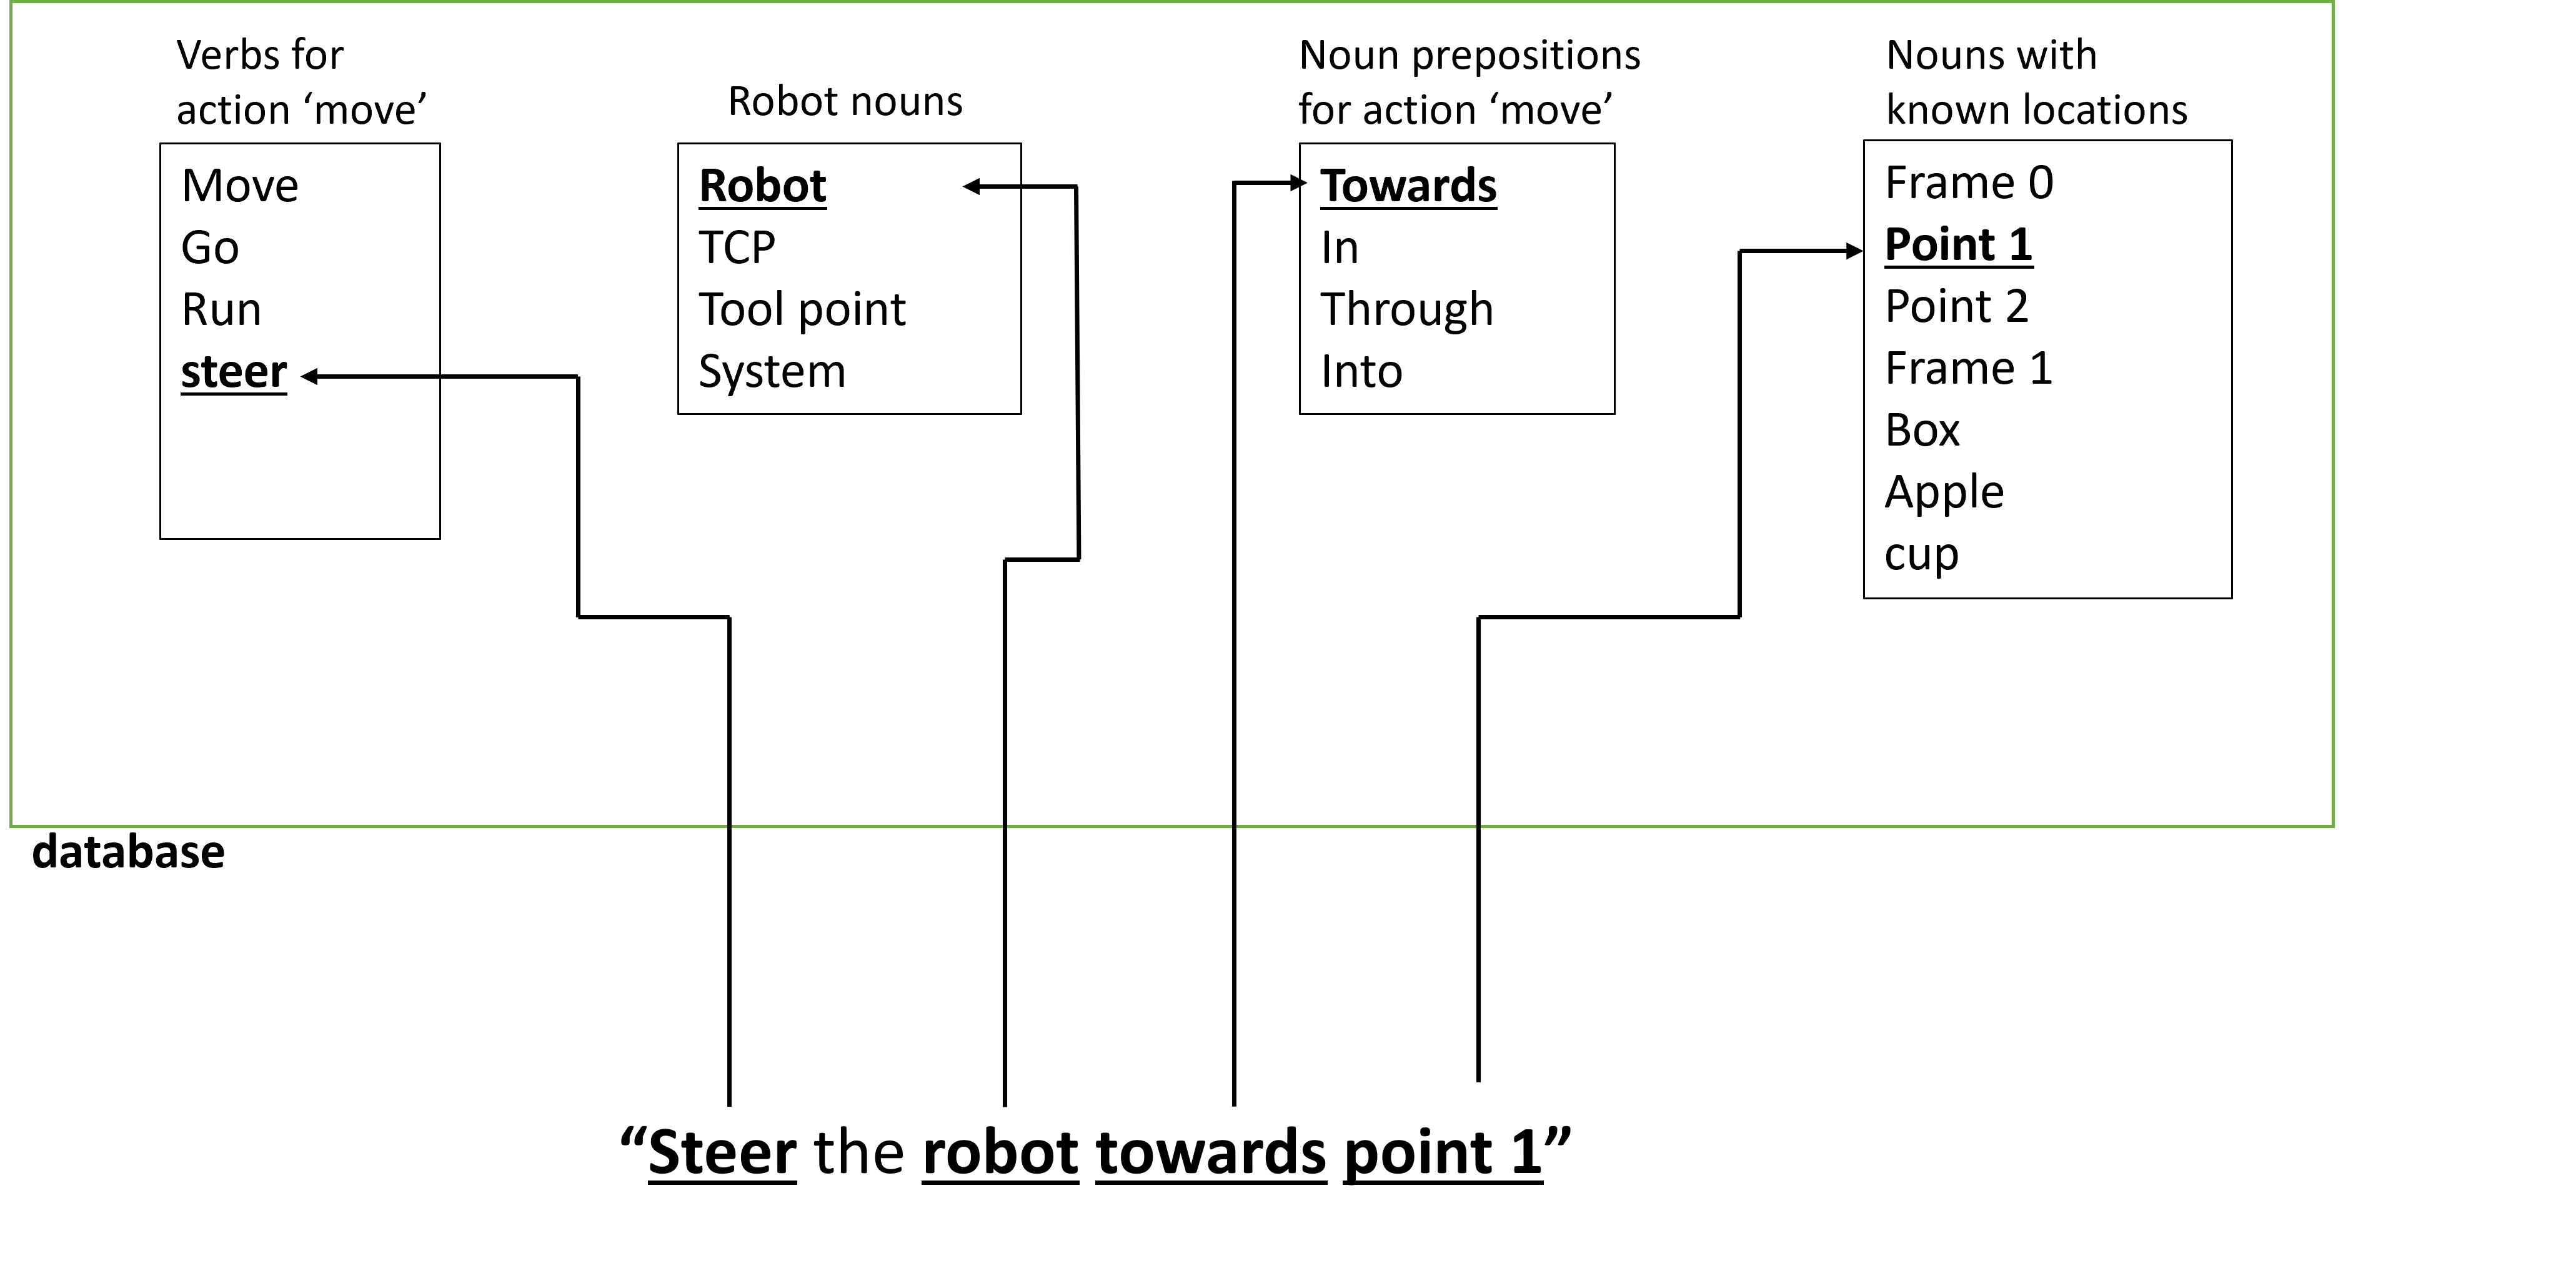
\includegraphics[width=14cm]{img/database_example.png}
    \caption{Figure illustrating an example of how the database works.}
    \label{fig:verb_sentence_move_box_PDF}
\end{figure}
The other type of information is the location of points and frames. This information is used in the kinematics pipeline to move the robot. The location information of points is stored as vectors denoting position, and frames are stored as homogenous transformations.
It is determined that the database is a tree structure with .txt files, as this structure is practical for fast reading and writing.

\section{Word comparison using cosine similarity} \label{sec:comp_method}
An NLP tool is used for the comparison of input words with database words. This tool is used to catch errors when the input words do not match any words in the database. Like using 'proceed' as a synonym for 'move'. Also, if the system is not constrained by the dictionary of words in the database, it would gain a larger corpus, which would increase the natural language interpretation ability.
Ideally, the system would not compare the words grammatically but rather with their intentions.
The comparison method used is therefore the cosine similarity of word embeddings. Which uses the dot product of two word embedding vectors to calculate their similarity. The similarity values go from -1 (no similarity) to 1 (full similarity). Figure \ref{fig:cosine_similarity_example} shows how the similarity score is used in this thesis. If the word used in the input does not match any words in the corresponding database word list, then the database word with the highest similarity score is suggested to the user. If the user disagrees, then the next highest similarity score option is given. This repeats until the user is satisfied or a threshold is reached, at which point the system gives up.
In chapter \ref{ch:eval} it is evaluated that the lowest similarity score needed to match all words in the data is $0.40$.

\begin{figure}[ht]
    \centering
    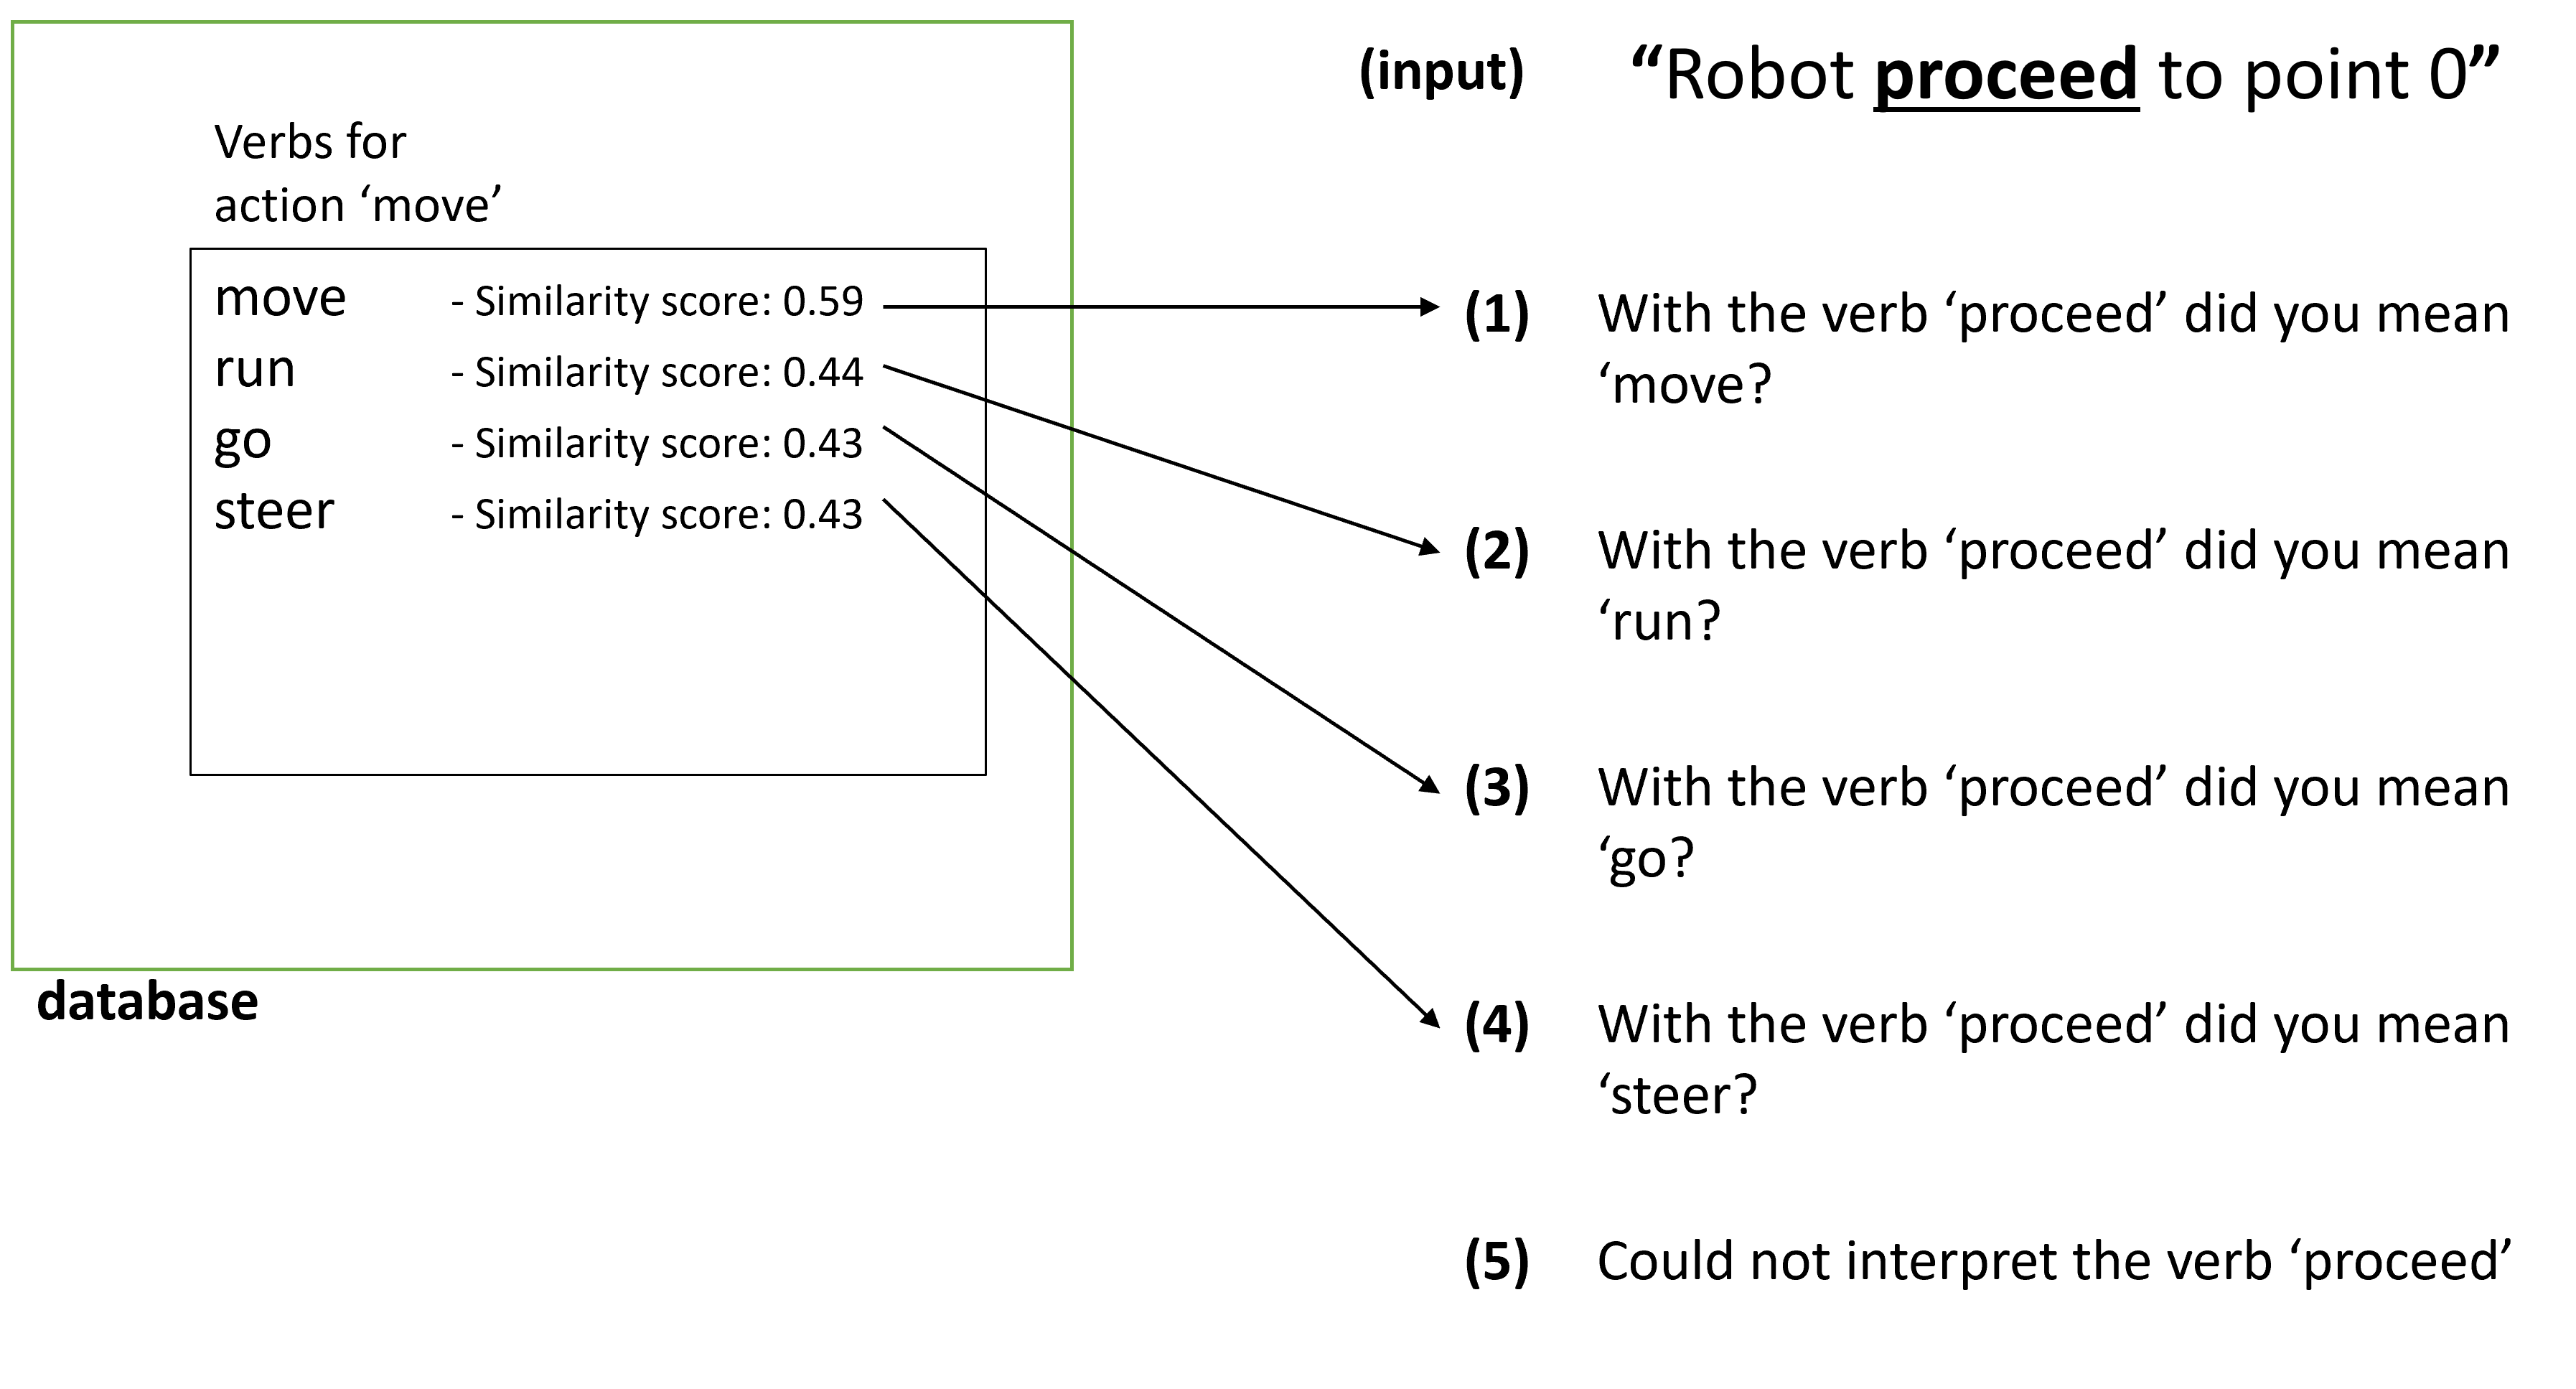
\includegraphics[width=14cm]{img/Cosine_similarity_example.png}
    \caption{Figure illustrating how the cosine similarity is used to communicate with the user.}
    \label{fig:cosine_similarity_example}
\end{figure}

\section{Parsing NLP pipeline output to actions} \label{sec:decon}
The earlier sections describe methods used to process individual words. The database holds the words matched with the words in the input sentence to find actions. The cosine similarity communicates with the user if any input words do not match the words in the database. It would be impractical to match all words in the database with all words in the sentence. It is therefore necessary to analyze the NLP pipeline output to gain more information about the words in the sentence before matching the words with the database words.
Figure \ref{fig:dep_pars_Parser} shows a visualization of the information gained by the NLP pipeline output. Firstly, it is known that the verb-by-verb relation 'parataxis' is used to split the sentence into its several instructions. Afterward, the root of each instruction is matched with the action verbs in the database, as the root is always a verb. The nouns connected to their respective root verbs are analyzed to find the information needed to execute the actions. The analysis methods for the nouns are action-specific. It is therefore explained in the later sections.
\\\\
Using the comparisons method explained previously and using the information gained from the NLP pipeline, the sentence in figure \ref{fig:dep_pars_Parser} can be transformed into two actions as shown in figure \ref{fig:dep_pars_actions}.


\begin{figure}[ht]
    \centering
    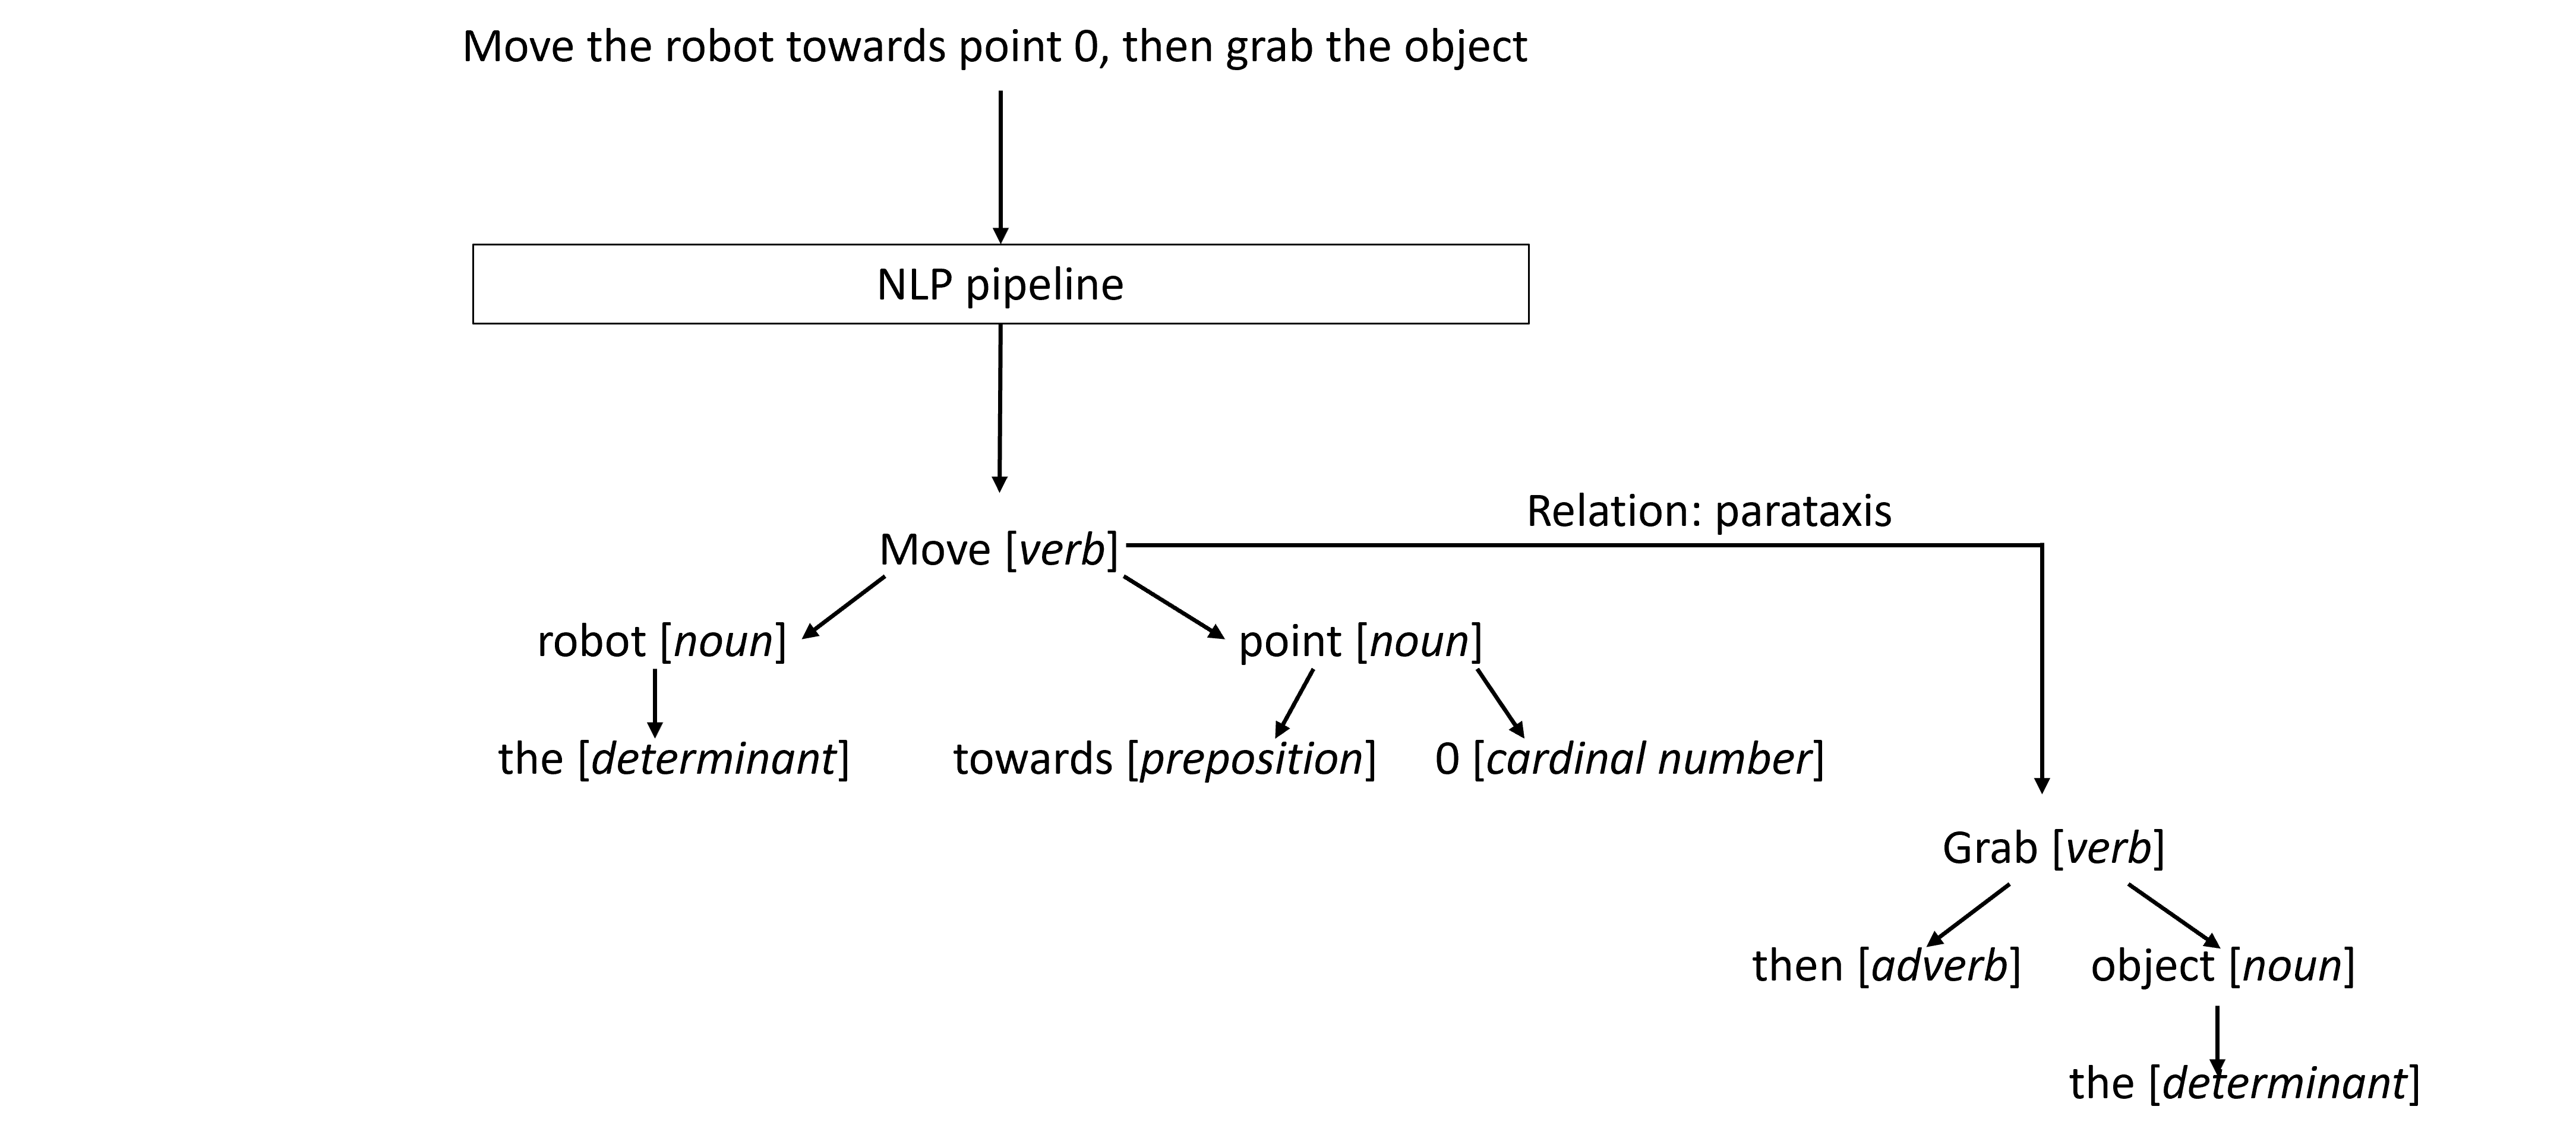
\includegraphics[width=14cm]{img/NLP_pipeline_output.png}
    \caption{Figure illustrating the NLP pipeline output from the previous chapter.}
    \label{fig:dep_pars_Parser}
\end{figure}

\begin{figure}[ht]
    \centering
    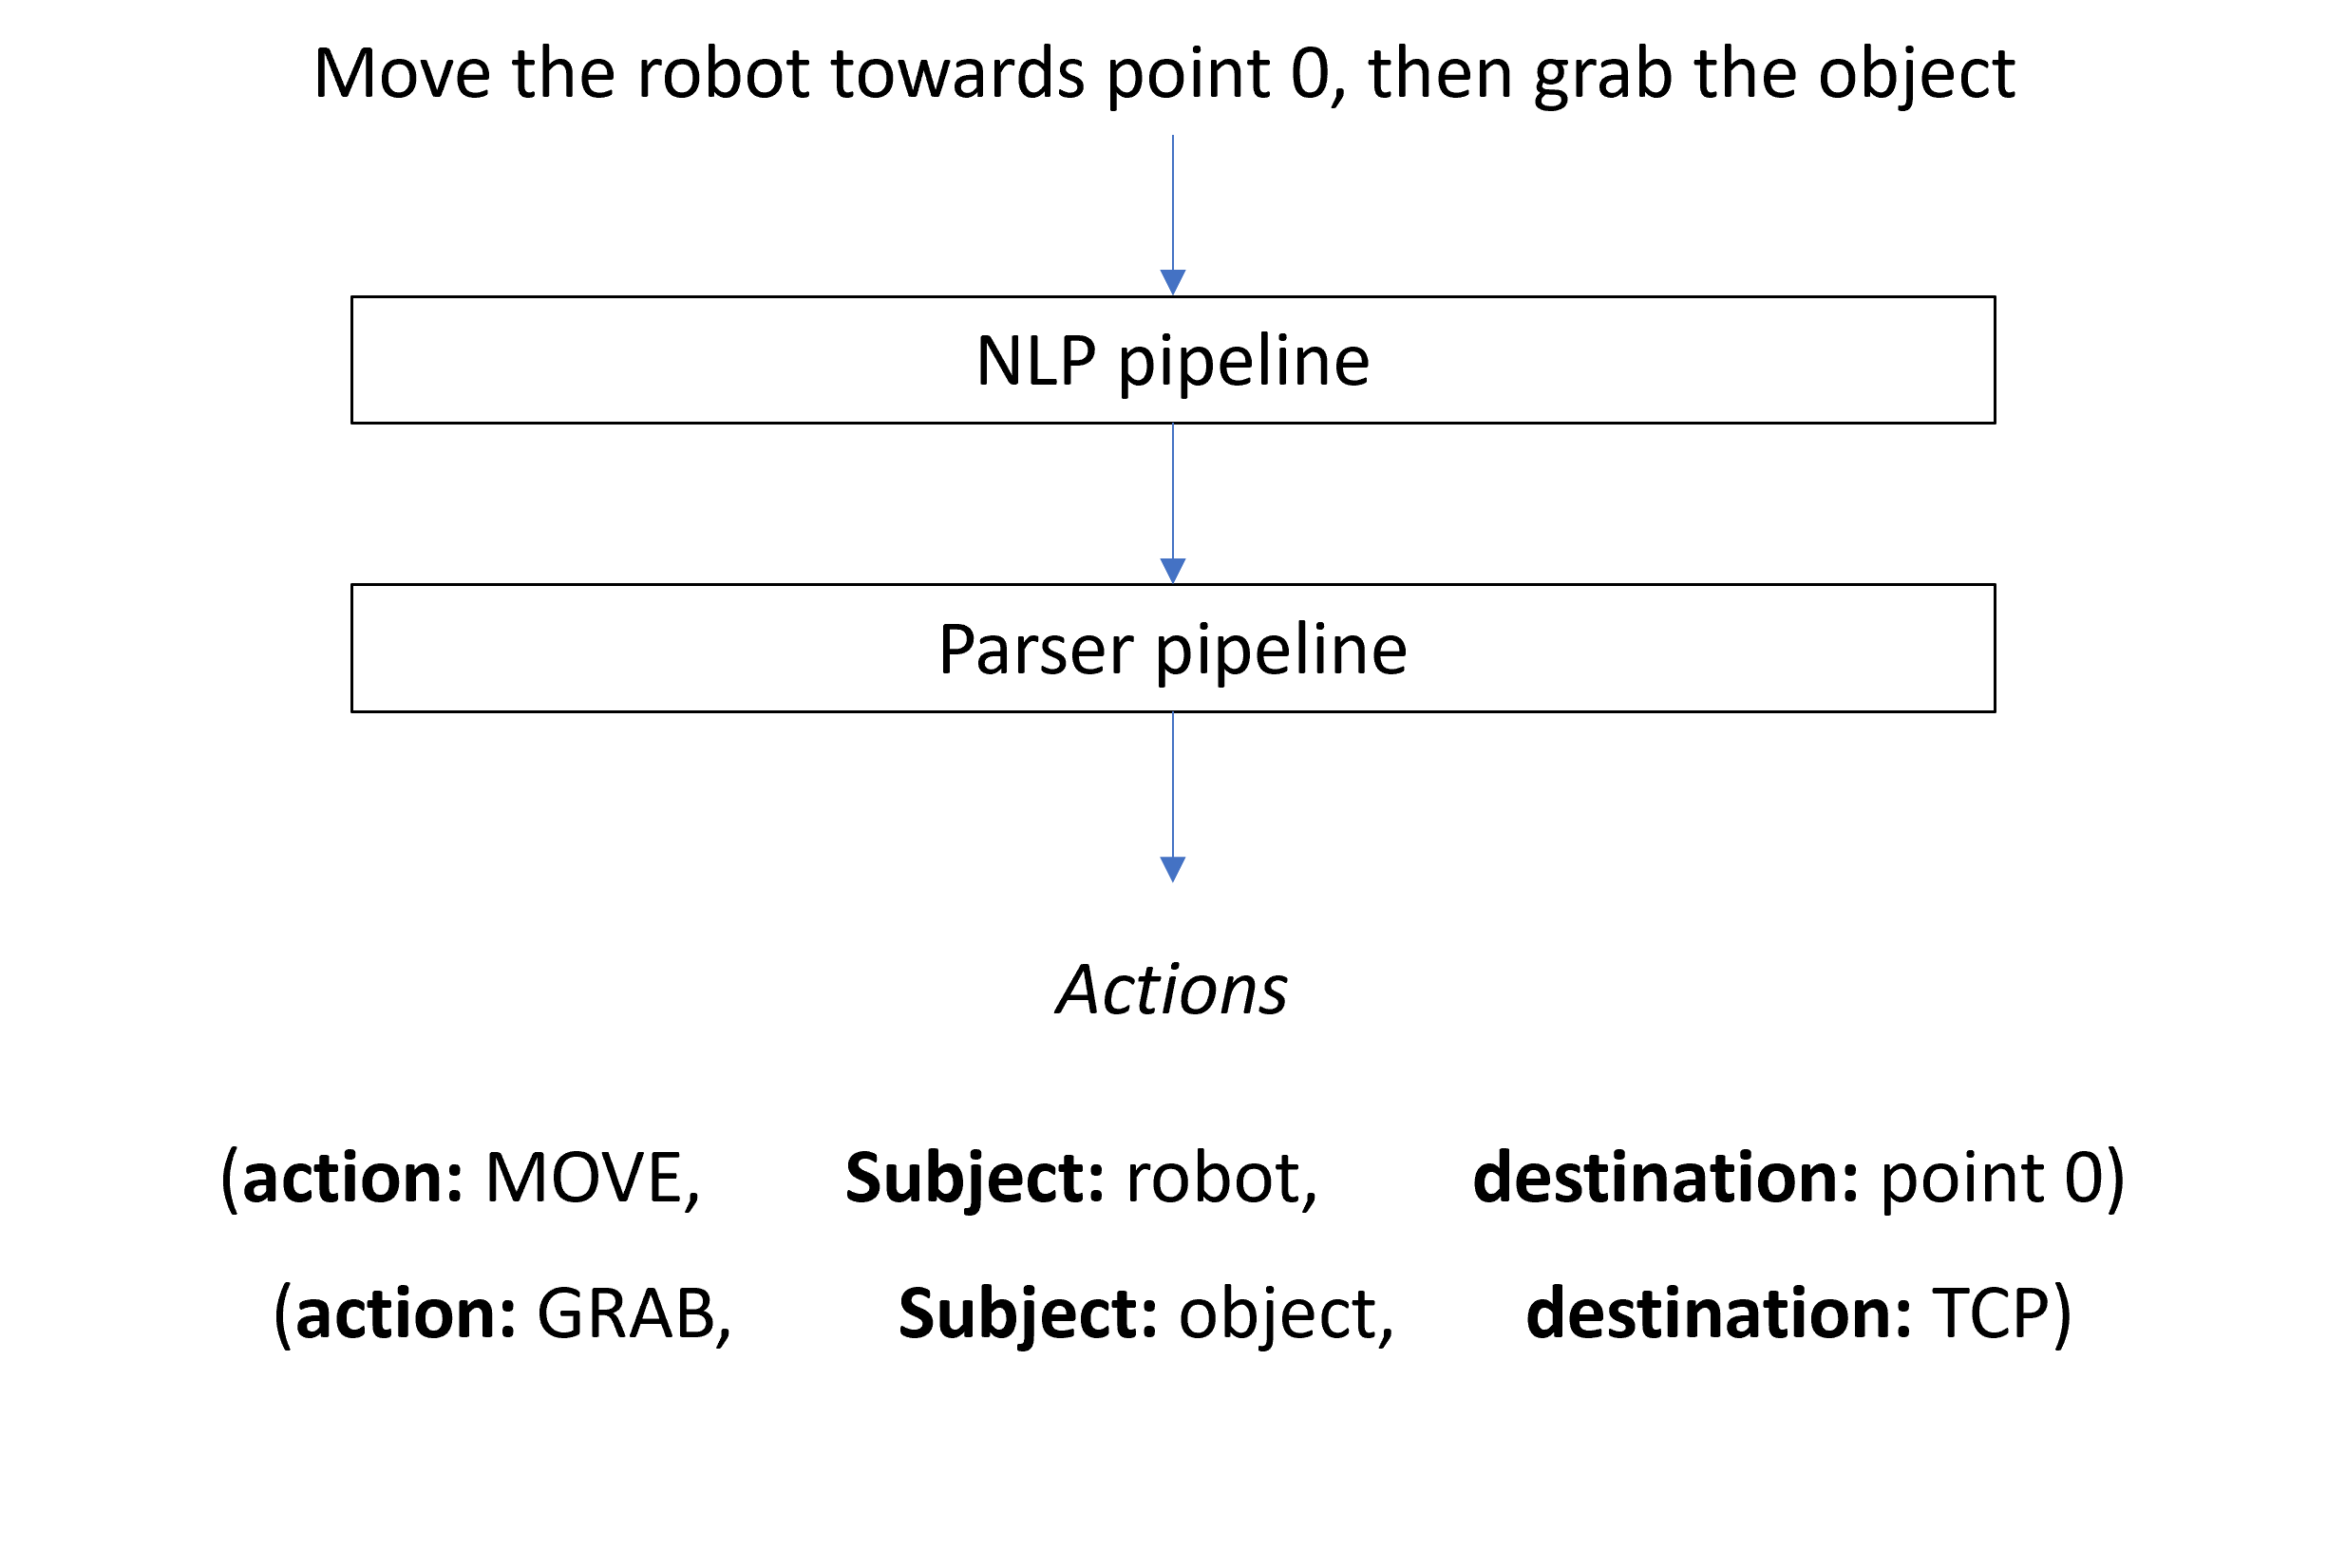
\includegraphics[width=10cm]{img/dep_parser_to_actions.png}
    \caption{Figure showing the parser pipeline output as actions.}
    \label{fig:dep_pars_actions}
\end{figure}



\section{Actions}
The last part of the parser pipeline is the development of the actions. The actions are designed to move the robot manipulator so that it is capable of solving tasks. The key is making the actions simple so that all tasks are a concatenation of them, as described by the user.
The action objects are divided into three categories, movement actions, meta actions, and system actions. The movement actions describe a robot's movement. The meta actions manipulate the sequence of actions. The system's actions manipulate points and frames in the physical environment. Meta actions are resolved in the pipeline before sending the list of actions to the kinematics pipeline. A list of the actions available is given below.
\begin{itemize}
    \item move
    \item rotate
    \item pick up
    \item put down
    \item repeat - Meta action
    \item set point or frame - System action
\end{itemize}
An in-depth description of each action, along with a visualization of the action objects, is given in the following sections.


\subsection{Action: Move} \label{esc:SA_MOVE}
The move action is split into the following two movement types:
\begin{itemize}
    \item Movement with reference to a point in space
    \item Movement relative in an axis
\end{itemize}

The first type describes the movement of the robot, based on points or frames in space.
The second type of movement describes how the robot should move if it is given a direction and a length. An example of this type of movement is \textit{'move 20 cm in the x-axis'}.
It is only capable of moving along the axes of the robot TCP.
The action object passed on is given as a list written as in figure \ref{fig:action_obj}.
\begin{figure}[ht]
    \centering
    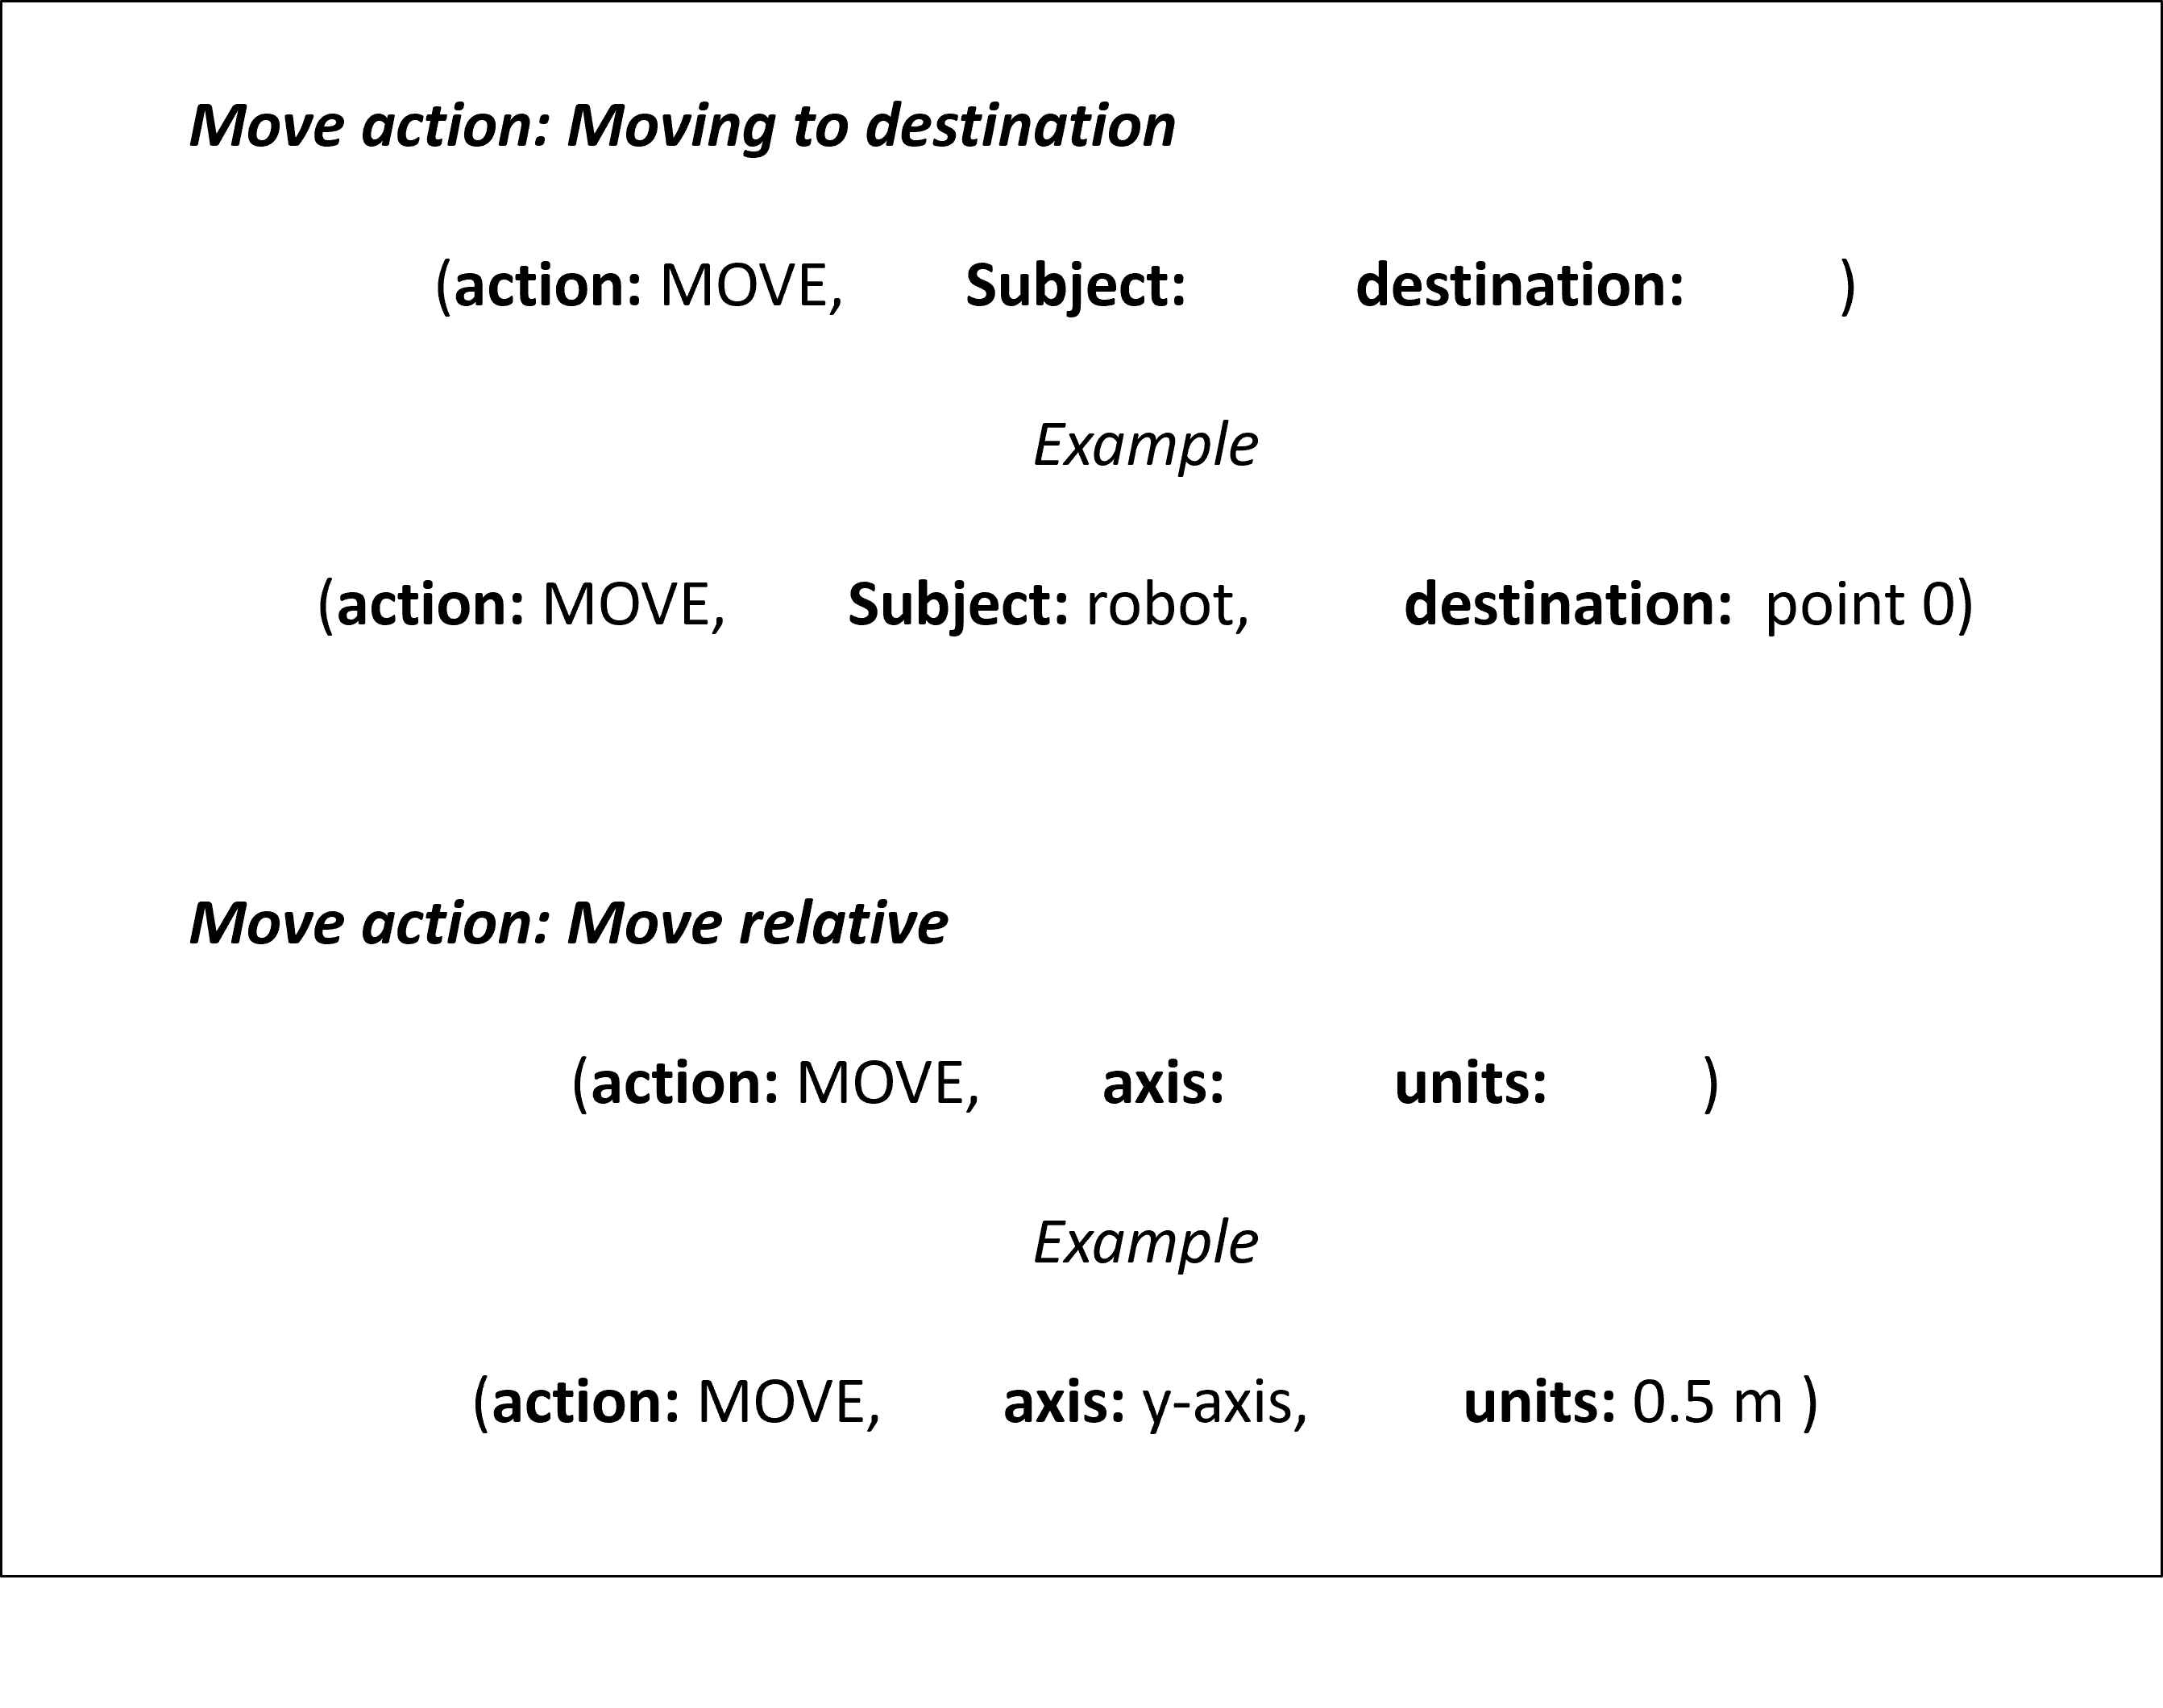
\includegraphics[width=10cm]{img/action_obj.png}
    \caption{Figure illustrating how the 'move' action would look in the system.}
    \label{fig:action_obj}
\end{figure}
\\\\
For the action 'move' specified by destination, then the subject of the movement is found by searching the NLP input for a noun without a preposition as in the word 'robot' in figure \ref{fig:dep_pars_Parser}. Afterward, the noun is also checked in the database to make sure it is valid and that it is not a random noun in the sentence. The destination is found by searching the sentences for a noun with a preposition. In figure \ref{fig:dep_pars_Parser} it can be seen that the noun 'point' has a preposition 'towards' that furthermore also matches the prepositions in the database for noun destinations of the action 'move'. This makes 'point' a destination for the action move in the example. The cardinal number '0' is observed to not always be connected with its noun. This is the reason for the solution of just treating cardinal numbers in front of the nouns 'point' and 'frame' as part of the noun.
\\\\
The action 'move' specified as a relative movement, is chosen if two conditions are met. If a noun describing one of the three frame axes is detected, And if no destination noun is found. Furthermore, the noun describing the axis must also have a preposition that shows that the action is done towards the axis noun. Examples of prepositions could be \textit{"along or using"}. If these conditions are met, then instead of searching for a noun destination, the system instead searches for a cardinal number along with units. An example could be \textit{"meters, m, centimeters, cm"}. After finding the axis and the cardinal number describing distance, it is passed on as an action.
\\
It should also be noted, that if no noun subject is found, then it is by default 'robot'. Such as in the sentence \textit{'move to point 0'}.



\subsection{Action: Pick up/Put down} \label{esc:SA_Pickup}

Though picking up and putting down are two separate actions, it makes more sense to treat them as a pair. Kinematically, they have no influence, as these actions control the gripper. The system is capable of remembering the objects it is holding, so it does not try to pick up objects when it is already holding one. As of now, no real objects are coded into the system, meaning that only the default object called "object" is available. The system is capable of supporting a design where each object has its own coordinate in space. But this work is left for future work.
The destination space in figure \ref{fig:action_PUT_PICK} is if the grab is done at a specific location, as with the sentence \textit{'pick up the object at point 0'}.

\begin{figure}[ht]
    \centering
    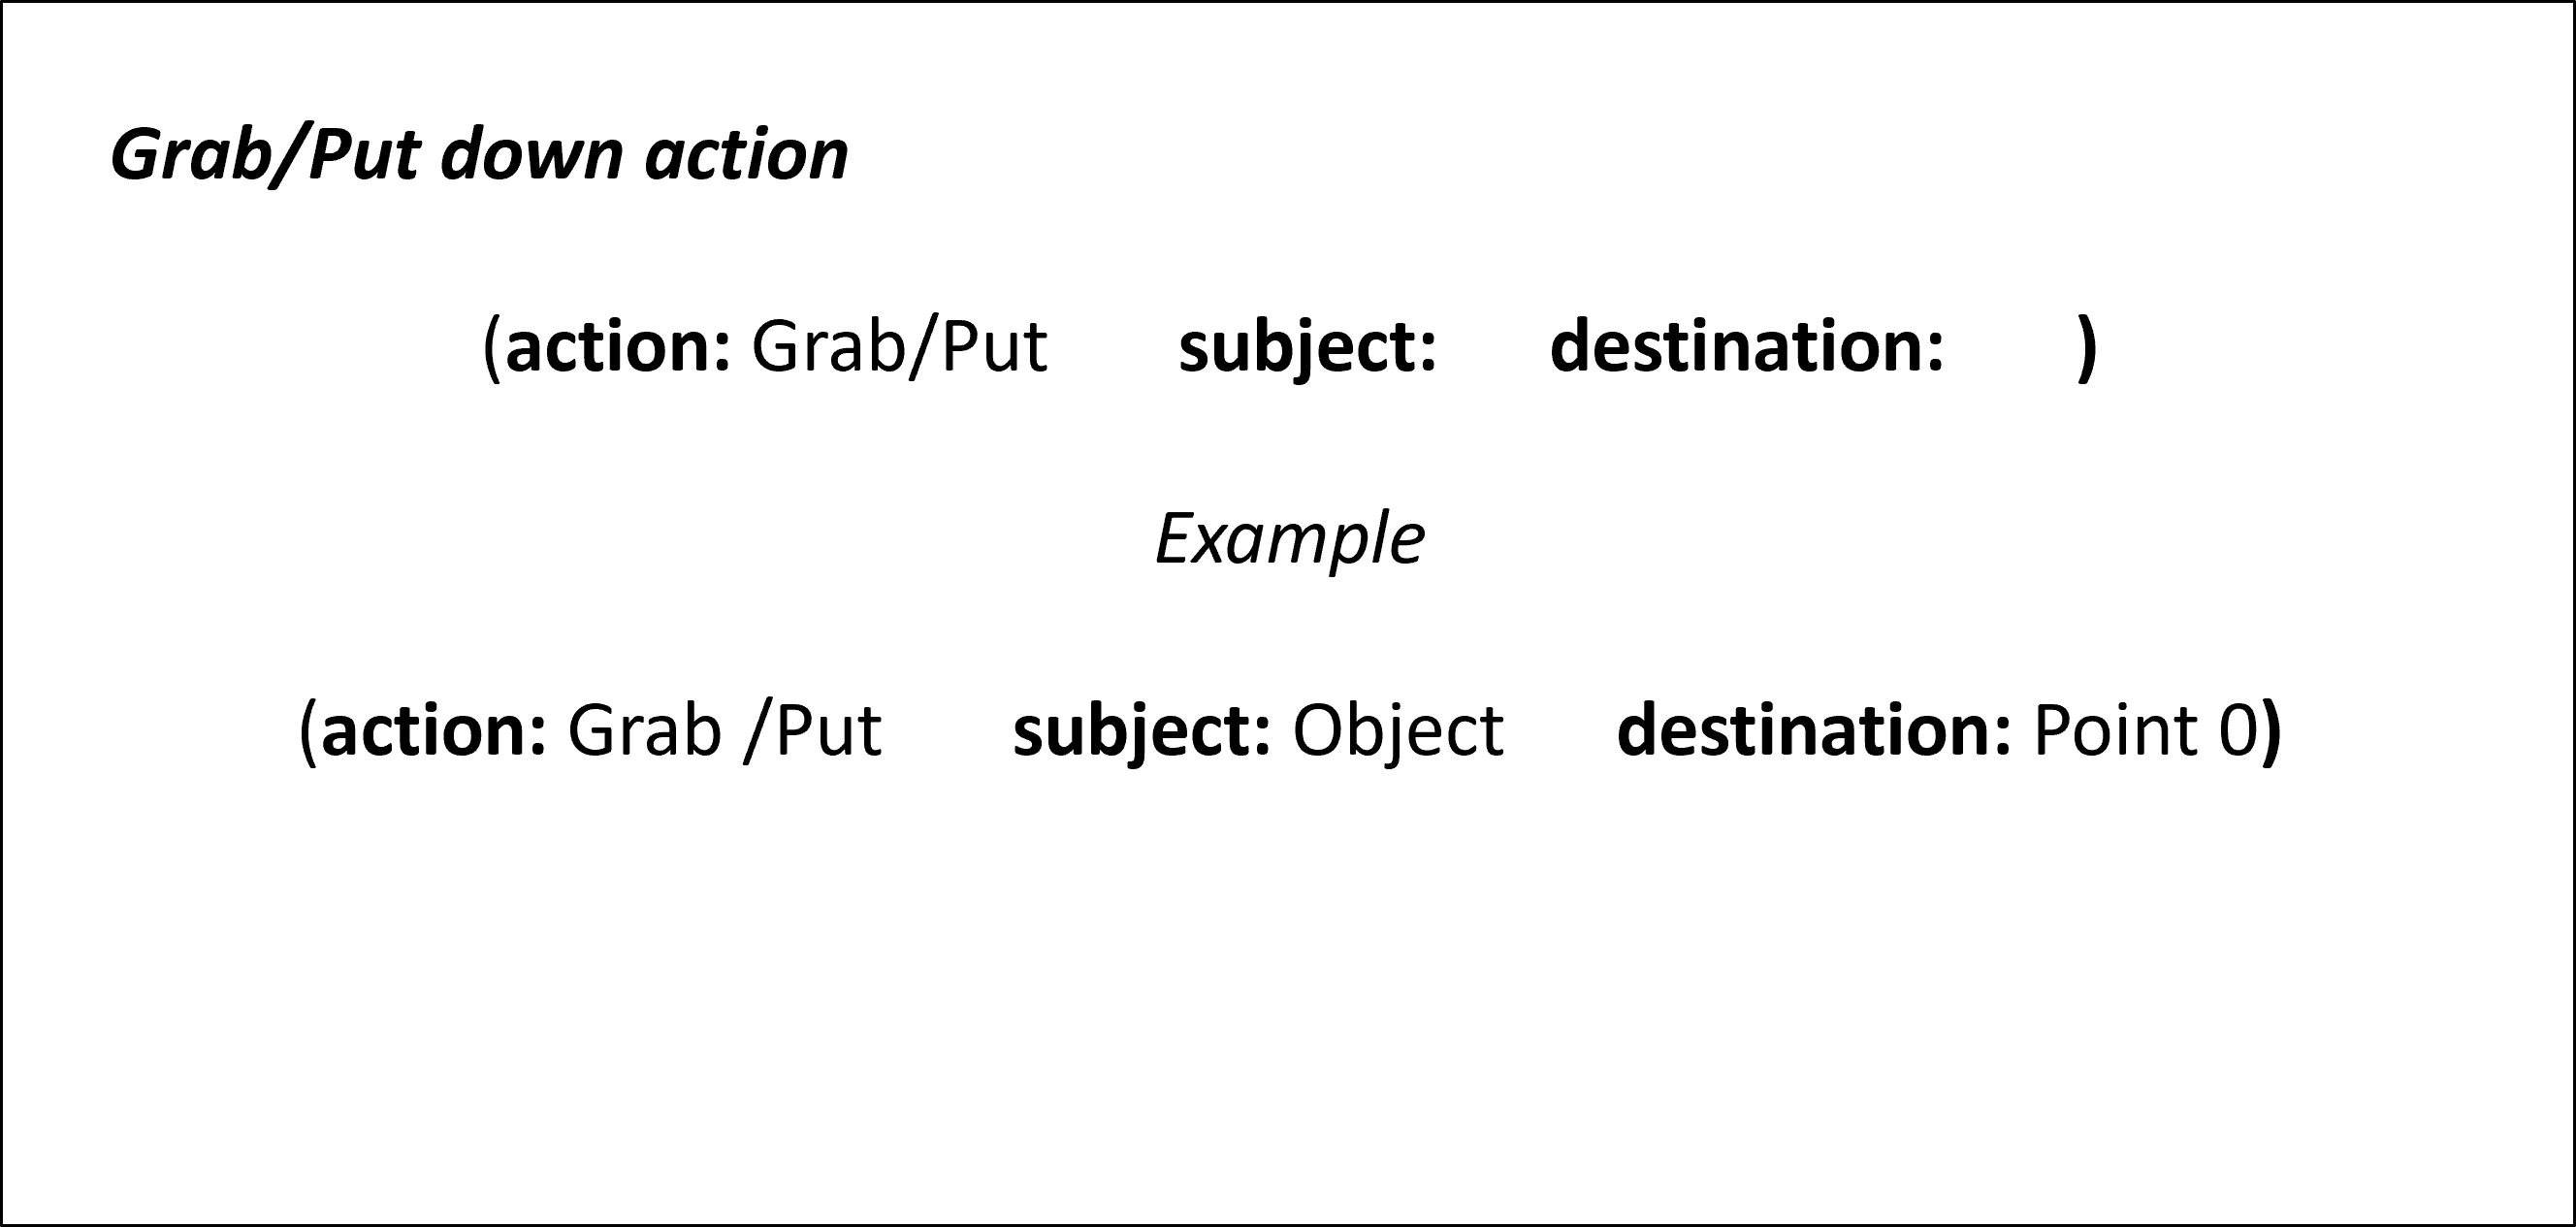
\includegraphics[width=10cm]{img/Put_Pick_obj.png}
    \caption{Figure illustrating how the put/pick action would look in the system.}
    \label{fig:action_PUT_PICK}
\end{figure}
The system finds the subject by searching the instruction for a noun without a preposition. The words found are checked in the database to make sure they are valid.
The destination is found by searching for a noun with a preposition, exactly the same as with the move action.
The destination noun is, per default, TCP. and the subject is, by default, the object "object". Therefore, a valid sentence for picking up or putting down could simply be \textit{'pick up'} or \textit{'put down'}. where the noun subject would be 'object' and the noun destination would be 'TCP'.



\subsection{Action: Rotate} \label{esc:SA_ROT}
As the UR5e robot only has revolute joints, this action is made with the intention of manipulating any part of the robot. An example of an instruction with the rotate action could be \textit{'\textit{rotate 90 degrees around wrist 3}'}.
The action object created is given in figure \ref{fig:action_ROT}.

\begin{figure}[ht]
    \centering
    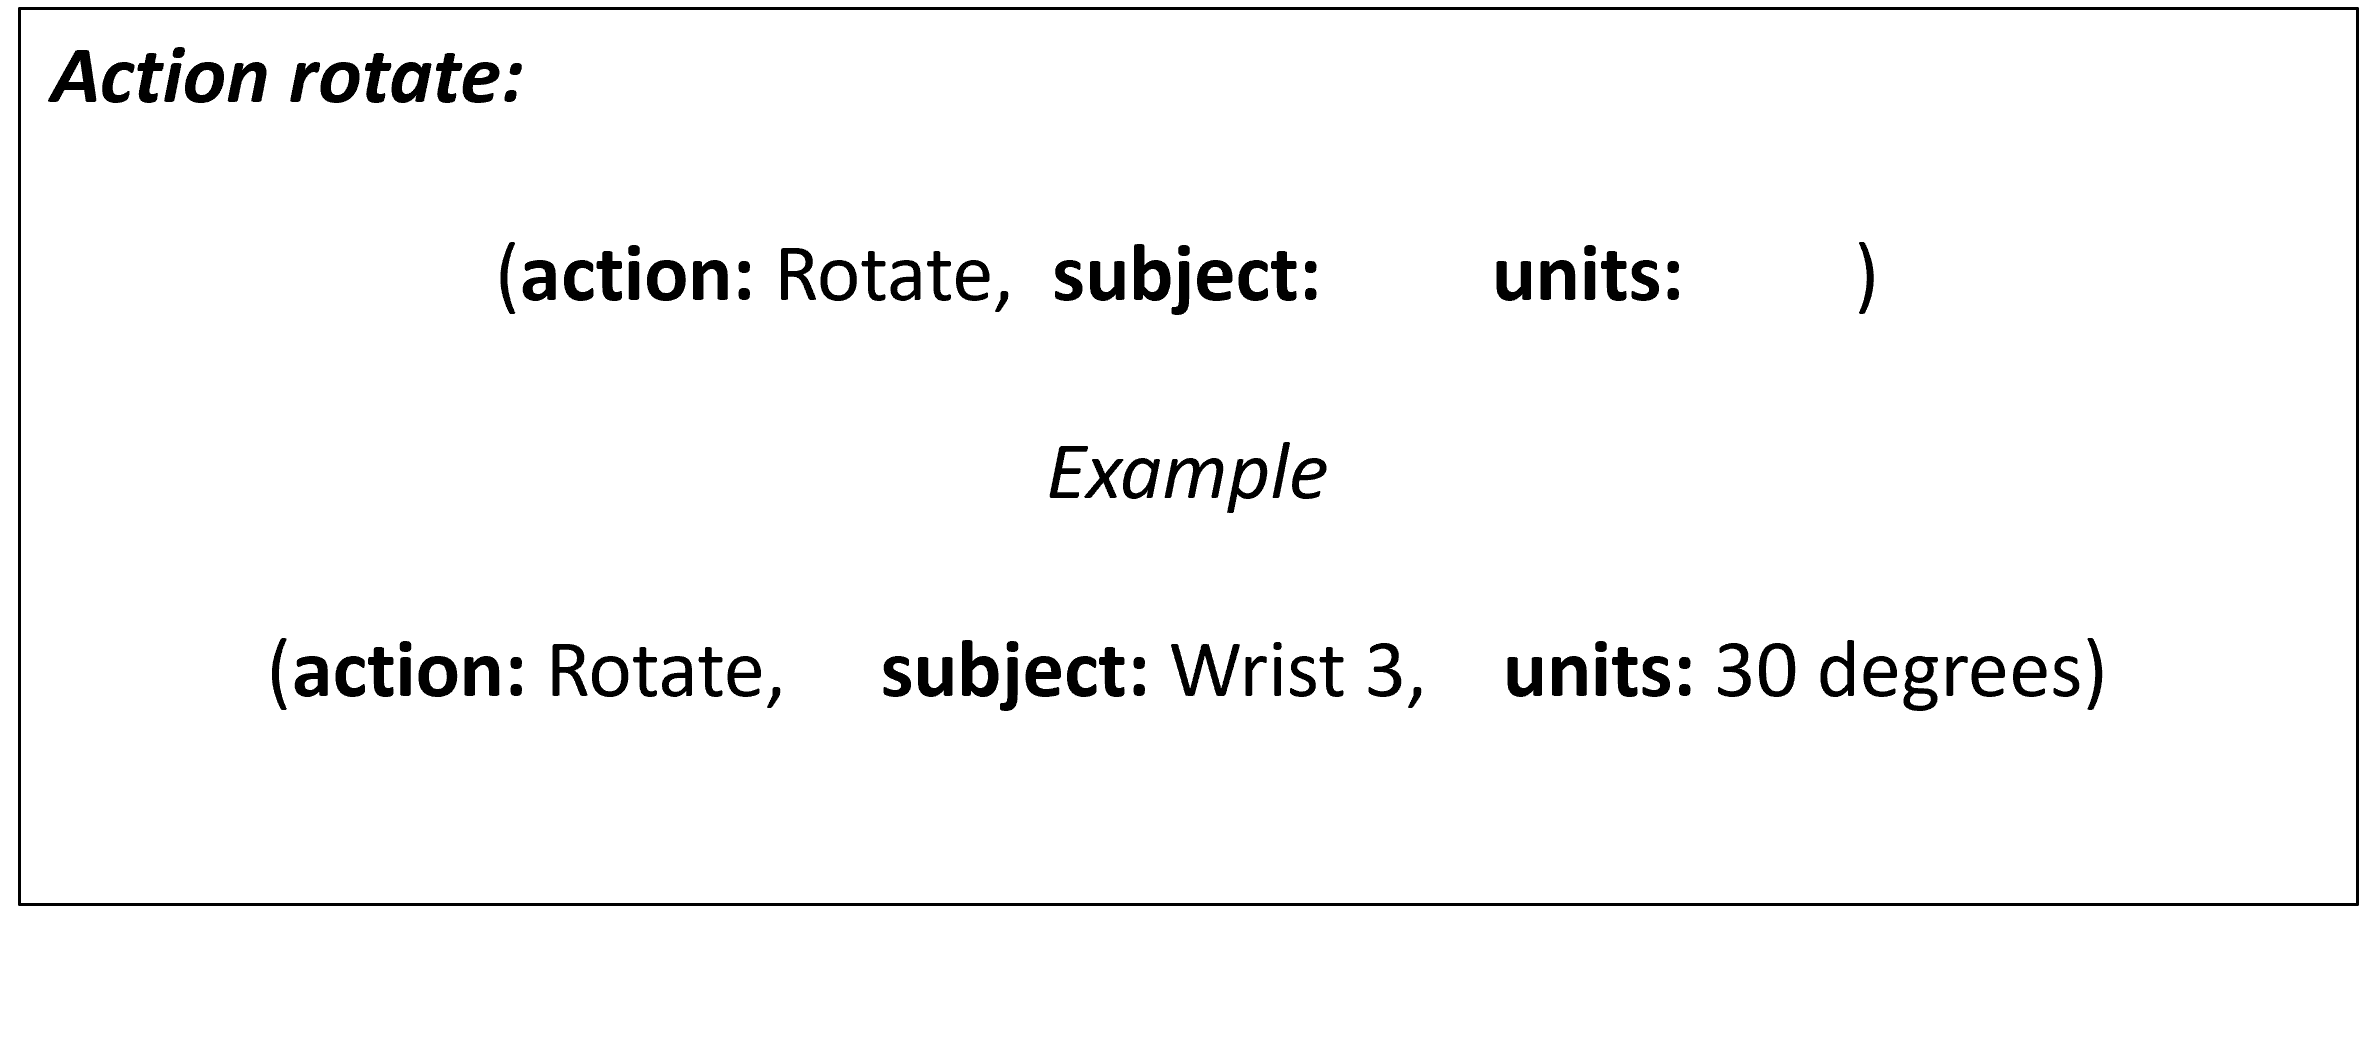
\includegraphics[width=10cm]{img/action_ROTATE.png}
    \caption{Figure illustrating how the rotate action would look in the system.}
    \label{fig:action_ROT}
\end{figure}

The subject of the action is found by searching for a noun (with or without prepositions) that corresponds to a part of the UR5e robot. The units are found the same way as the units are found in the action move relative. The subject is by default set to 'robot'. Meaning that the sentence \textit{'rotate 90 degrees'} would be interpreted as rotating the base of the robot 90 degrees.


\subsection{Action: Repeat} \label{esc:SA_REPEAT}
Repeat is a meta action, meaning that it serves to manipulate other actions while the system translates verb sentences into actions.
There are three types of repeat actions. Either it repeats the actions in the previous part of the sentence, the next part of the sentence, or the whole sentence, regardless of the statement's position. The correct type of repetition action is determined based on the preposition bound to the subject of repetition. An example could be the following sentence \textit{'repeat the next actions 3 times'}.
where the repeat statement would repeat the next actions. But substituting the preposition 'next' with 'previous', would make the repeat statement repeat the previous actions. The action refers to all actions in the sentence if it cannot detect the use of either preposition hinting towards repeating either previous or next actions. The action object is shown in figure \ref{fig:action_REP}.

\begin{figure}[ht]
    \centering
    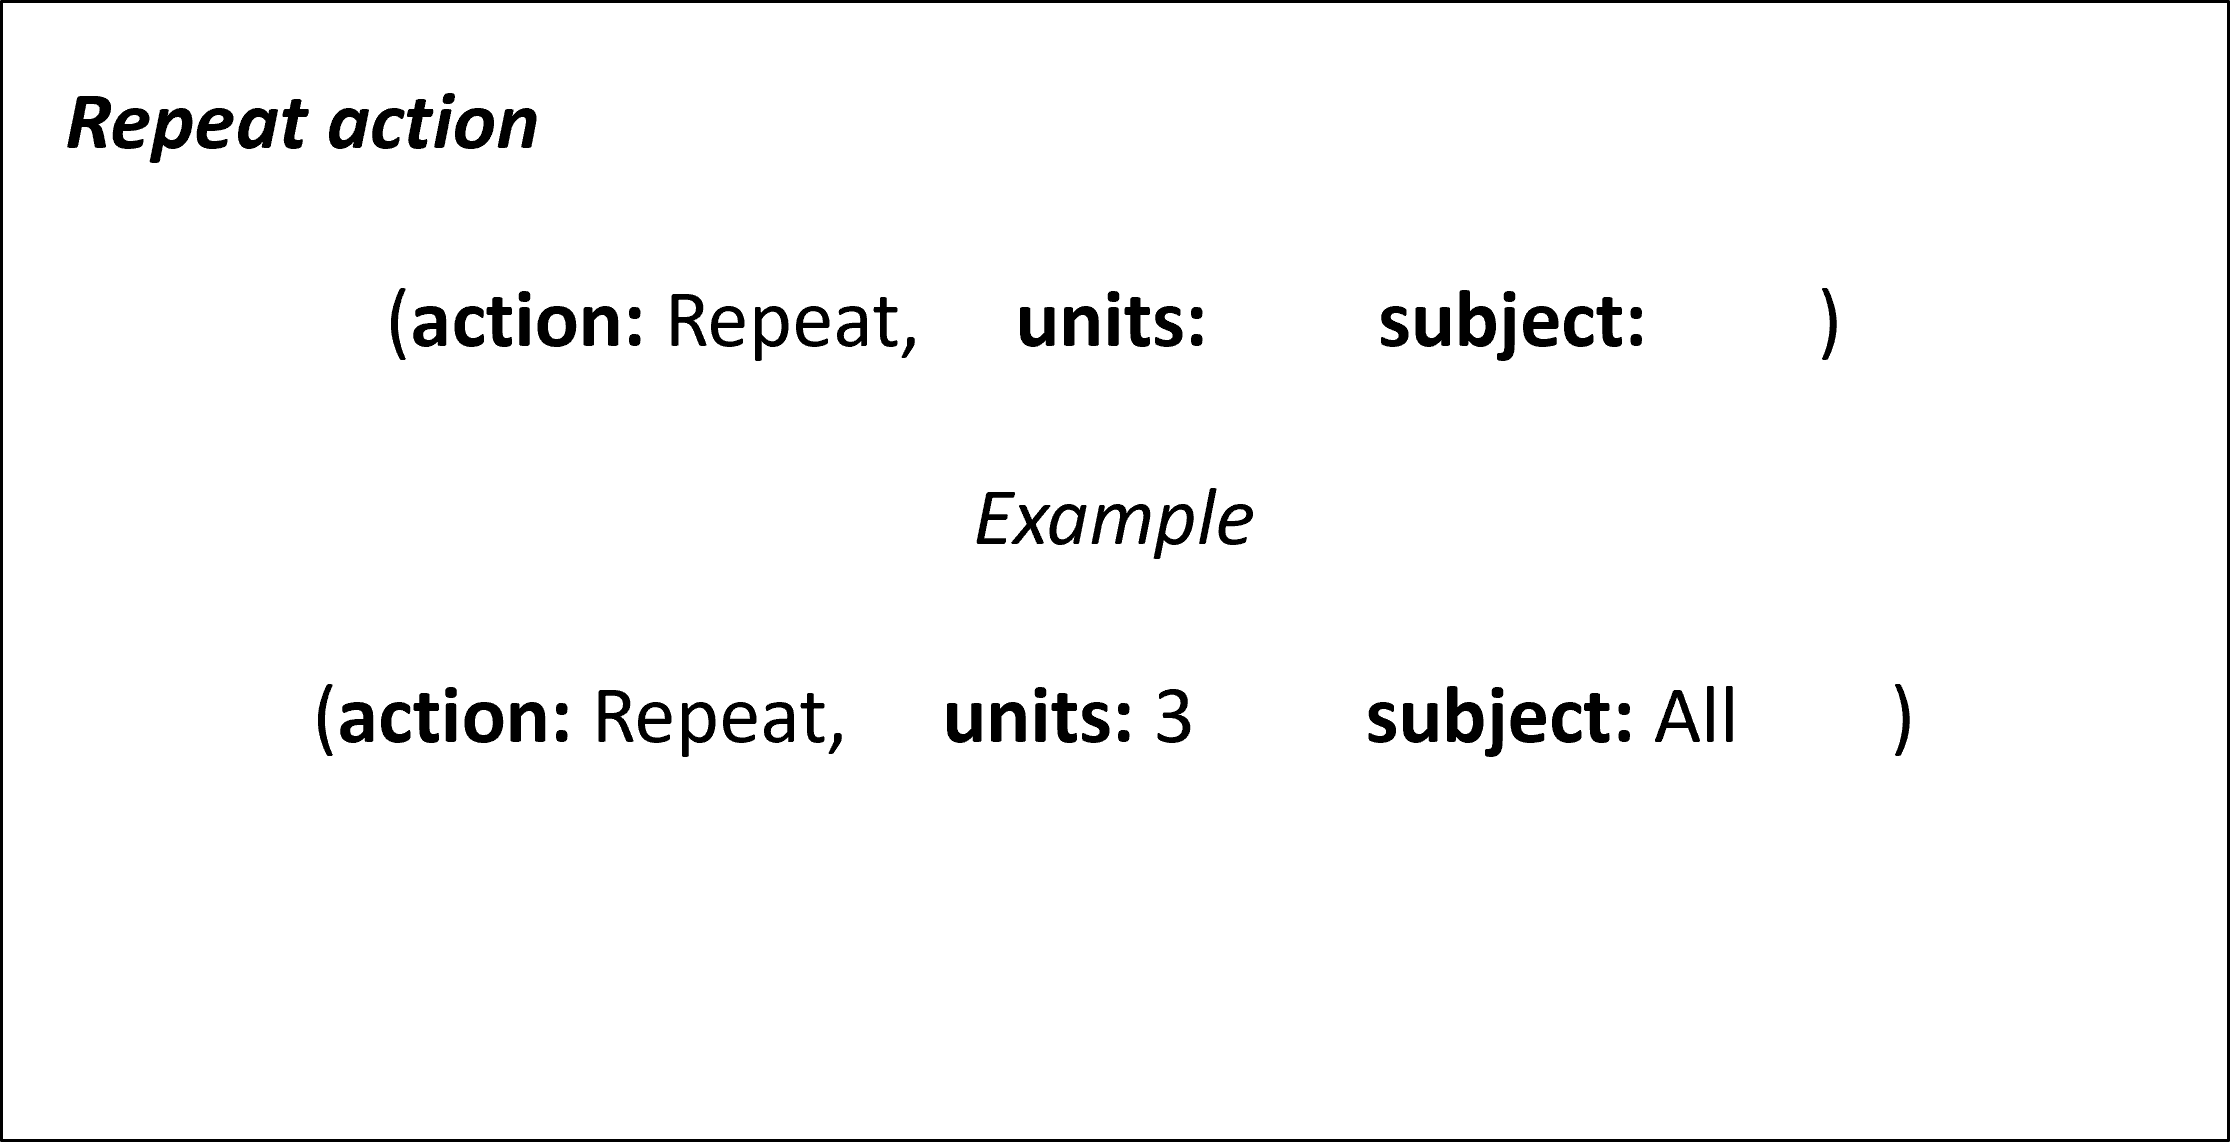
\includegraphics[width=10cm]{img/repeat_action.png}
    \caption{Figure illustrating how the repeat action would be perceived in the system.}
    \label{fig:action_REP}
\end{figure}

The units are found by searching for a noun describing the repeat amount. Like the noun \textit{'times'} or \textit{'cycles'}. Then afterward use the number that comes before the unit. The subject is found as described in how the action is split into three categories.


\subsection{Action: set}\label{esc:action_set}
This action is a system action, meant for setting up the tasks in the environment. Even if it is the only system action, the versatility of the verb 'set' allows it to do three different things. Specifically, the things stated in the following list.

\begin{itemize}
    \item Store the position of the tool center point as a new point.
    \item Store the pose of the tool center point as a new frame.
    \item Switch the frame that the robot works in with another frame.
\end{itemize}

\begin{figure}[ht]
    \centering
    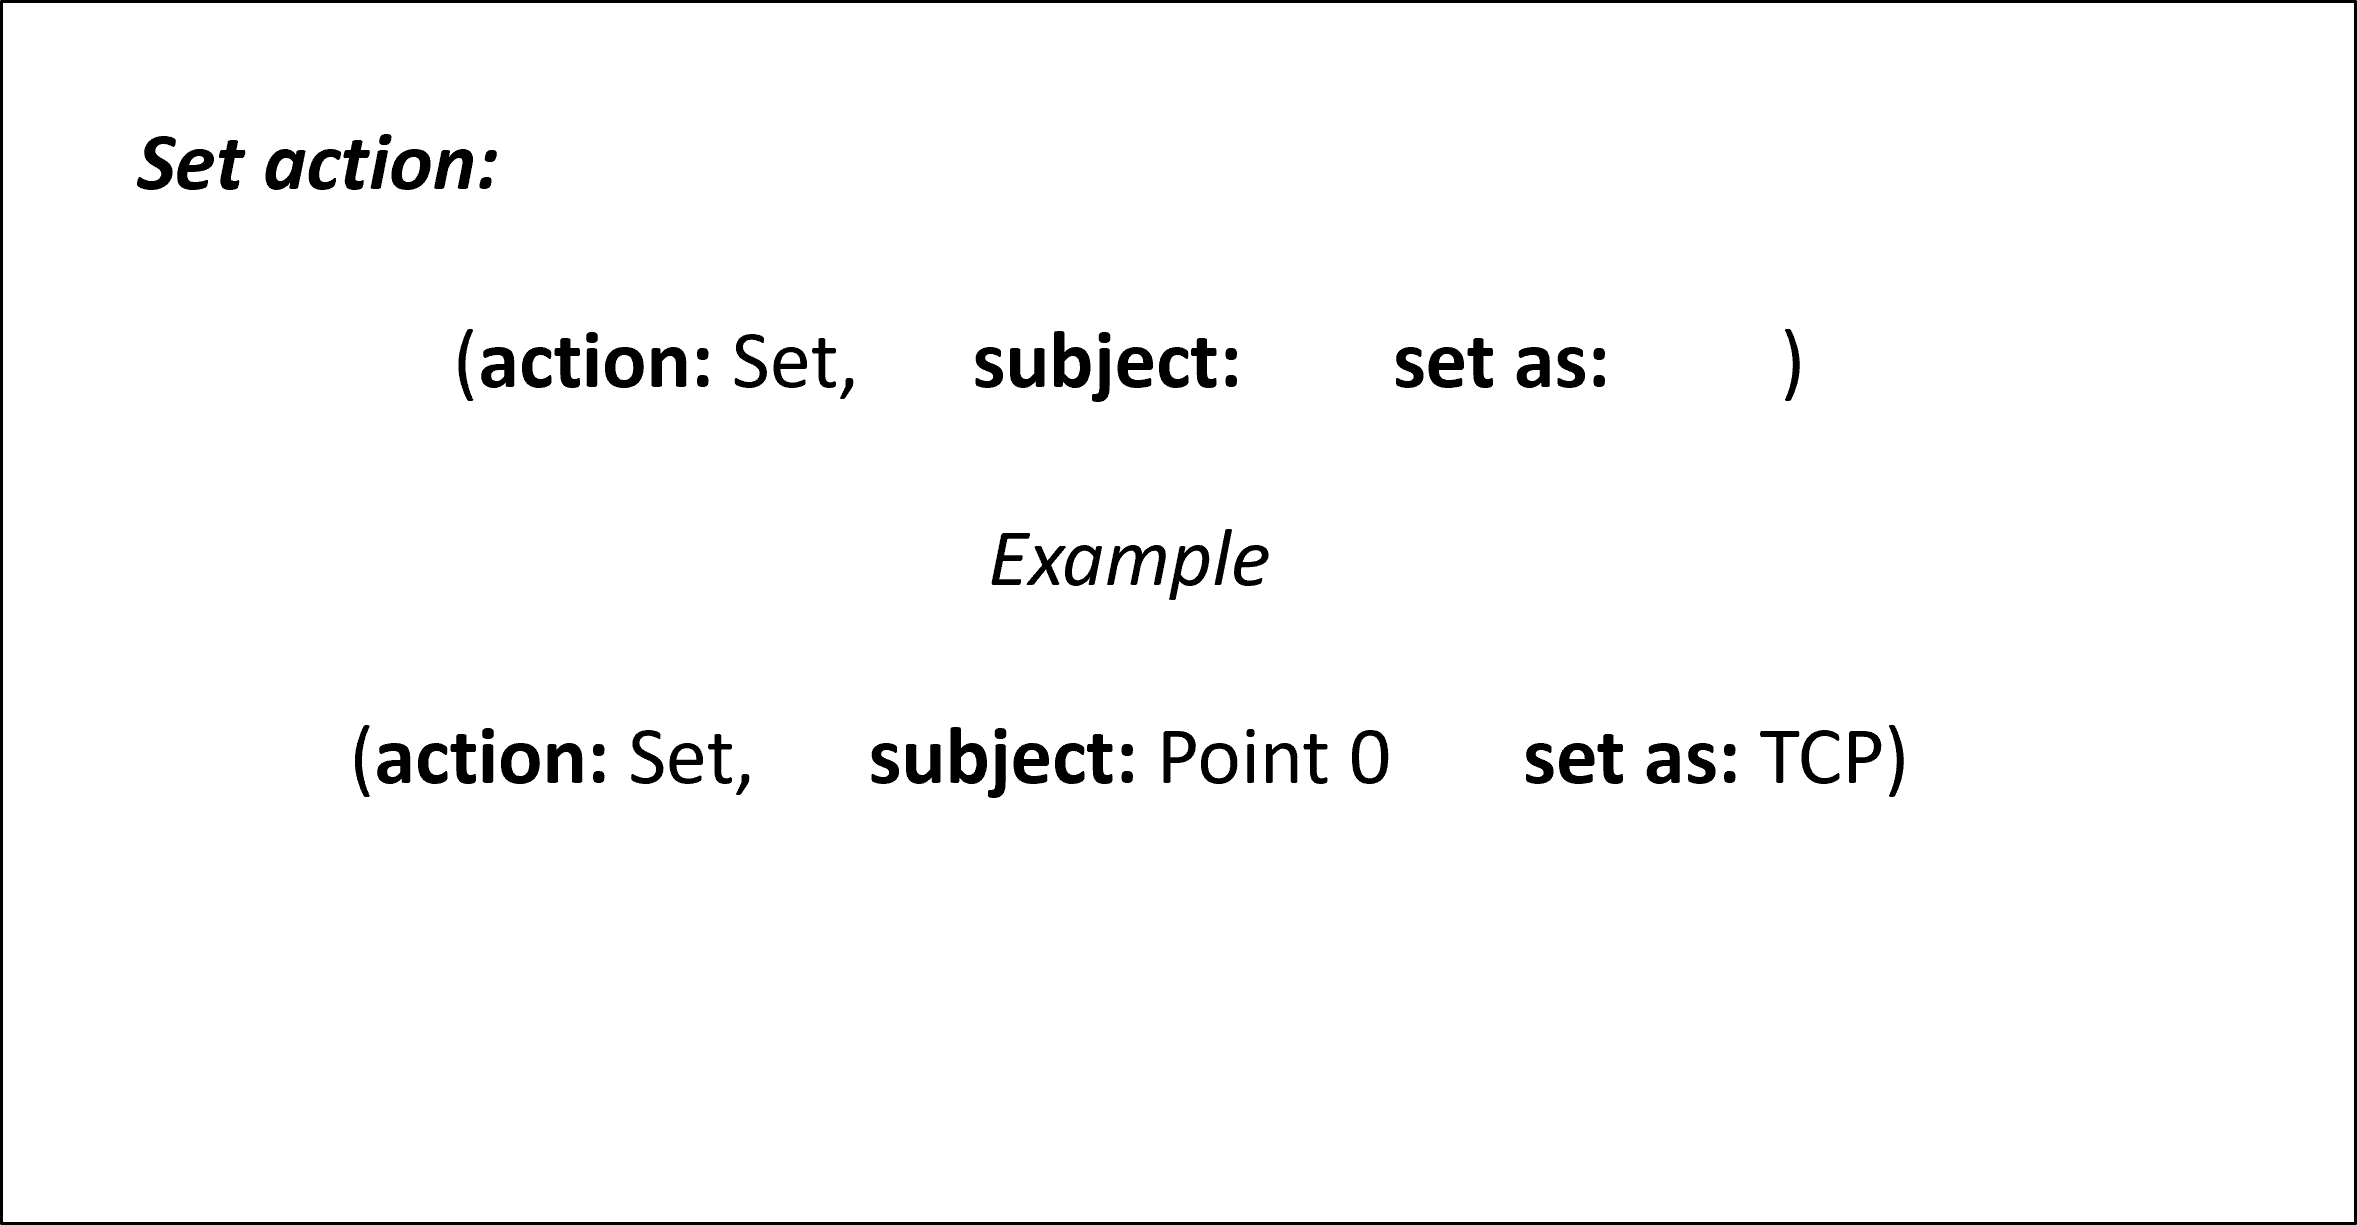
\includegraphics[width=10cm]{img/action_SET.png}
    \caption{Figure illustrating how the set action would be perceived in the system.}
    \label{fig:action_set}
\end{figure}
The set action is shown in figure \ref{fig:action_set}.

The subject is found by searching for a noun without a preposition. 'set as' is not processed and is always its default value, which is TCP. But the idea is that it could be used to set points at TCP + 7 cm on the z-axis. But this information is too complex and is therefore left for future work. If the noun subject is a frame with an index already present in the system, then the system switches the work frame to the new frame. If no index is given (both for the nouns 'point' and 'frame'), then a new 'point' or 'frame' is created.